\hypertarget{amk-results}{%
\section{Results}\label{amk-results}}

This section contains our results on the AK model, we first look at how we checked numerically that Lieb's theorem generalises to our model. Next we compute the ground state diagram and look at the two phases that arise there. We then use a local Chern marker and the presence of edge modes to characterise these phases as having Abelian or non-Abelian statistics. Finally we look at the finite temperature behaviour of the model.

\hypertarget{the-ground-state-flux-sector}{%
\subsection{The Ground State Flux Sector}\label{the-ground-state-flux-sector}}

We will check that Lieb's theorem generalises to our model by enumerating all the flux sectors of many separate amorphous lattice realisations. However, we have two seemingly irreconcilable problems. Finite size effects have a large energetic contribution for small systems~\autocite{kitaevAnyonsExactlySolved2006} so we would like to perform our analysis for very large lattices. For an amorphous system with \(N\) plaquettes, \(2N\) edges and \(3N\) vertices we have \(2^{N-1}\) flux sectors to check and diagonalisation scales with \(\mathcal{O}(N^3)\). That exponential scaling makes it difficult to work with lattices much larger than \(16\) plaquettes with the resources.

To get around this, we instead look at periodic systems with amorphous unit cells. For a similarly sized periodic system with \(A\) unit cells and \(B\) plaquettes in each unit cell where \(N \sim AB\) things get much better. We can use Bloch's theorem to diagonalise this system in about \(\mathcal{O}(A B^3)\) operations, and more importantly there are only \(2^{B-1}\) flux sectors to check. We fully enumerated the flux sectors of \(\sim\) 25,000 periodic systems with disordered unit cells of up to \(B = 16\) plaquettes and \(A = 100\) unit cells. However, showing that our guess is correct for periodic systems with disordered unit cells is not quite convincing on its own as we have effectively removed longer-range disorder from our lattices.

The second part of the argument is to show that the energetic effect of introducing periodicity scales away as we go to larger system sizes and has already diminished to a small enough value at 16 plaquettes, which is indeed what we find. From this, we argue that the results for small periodic systems generalise to large amorphous systems. In the isotropic case (\(J^\alpha = 1\)), Lieb's theorem correctly predicts the ground state flux sector for all of the lattices we tested. For the toric code phase (\(J^x = J^y = 0.25, J^z = 1\)) all but around (\(\sim 0.5 \%\)) lattices had ground states conforming to our conjecture. In these cases, the energy difference between the true ground state and our prediction was on the order of \(10^{-6} J\).

The spin Kitaev Hamiltonian is real and therefore has time reversal symmetry. However in the ground state the flux \(\phi_p\) through any plaquette with an odd number of sides has imaginary eigenvalues \(\pm i\). Thus, states with a fixed flux sector spontaneously break time reversal symmetry. Kiteav noted this in his original paper but it was first explored in a concrete model by Yao and Kivelson~for a translation invariant Kitaev model with odd sided plaquettes~\autocite{Yao2011}.

Flux sectors come in degenerate pairs, where time reversal is equivalent to inverting the flux through every odd plaquette, a general feature for lattices with odd plaquettes~\autocite{yaoExactChiralSpin2007,Peri2020}. This spontaneously broken symmetry serves a role analogous to the external magnetic field in the original honeycomb model, leading the AK model to have a non-Abelian anyonic phase without an external magnetic field.

\hypertarget{ground-state-phase-diagram}{%
\subsection{Ground State Phase Diagram}\label{ground-state-phase-diagram}}

The triangular \(J_x, J_y, J_z\) phase diagram of this family of models arises from setting the energy scale with \(J_x + J_y + J_z = 1\). The intersection of this plane and the unit cube is what yields the equilateral triangles seen in diagrams like \cref{fig:phase_diagram}. The KH model has an Abelian gapped phase in the anisotropic region (the A phase) and is gapless in the isotropic region. The introduction of a magnetic field breaks the chiral symmetry, leading to the isotropic region becoming a gapped, non-Abelian phase, the B phase.

Similar to the KH model with a magnetic field, we find that the amorphous model is only gapless along critical lines, see \cref{fig:phase_diagram} (Left). Interestingly, in finite size systems the gap closing exists in only one of the four topological sectors though the sectors become degenerate in the thermodynamic limit. Nevertheless, this could be a useful way to define the (0, 0) topological flux sector for the amorphous model which otherwise has no natural way to choose it.

In the honeycomb model, the phase boundaries are located on the straight lines \(|J^x| = |J^y| \;+ \;|J^z|\) and permutations of \(x,y,z\). These are shown as dotted lines in \cref{fig:phase_diagram} (Right). We find that on the amorphous lattice these boundaries exhibit an inward curvature, similar to honeycomb Kitaev models with flux or bond disorder~\autocite{knolle_dynamics_2016,Nasu_Thermal_2015,lahtinenPerturbedVortexLattices2014,willansDisorderQuantumSpin2010,zschockePhysicalStatesFinitesize2015,kaoDisorderDisorderLocalization2021}.

\hypertarget{fig:phase_diagram}{%
\begin{figure}
\centering
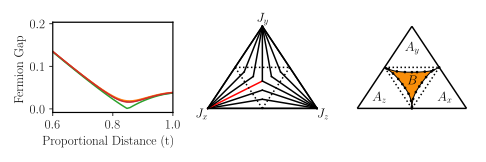
\includegraphics[width=1\textwidth,height=\textheight]{figure_code/amk_chapter/results/phase_diagram/phase_diagram}
\caption[{The Ground State Phase Diagram}]{The phase diagram of the model can be characterised by an equilateral triangle whose corners indicate points where \(J_\alpha = 1, J_\beta = J_\gamma = 0\) while the centre denotes \(J_x = J_y = J_z\). (Center) To compute critical lines efficiently in this space, we evaluate the order parameter of interest along rays shooting from the corners of the phase diagram. The ray highlighted in red defines the values of J used for the left figure. (Left) The fermion gap as a function of J for an amorphous system with 20 plaquettes, where the x axis is the position on the red line in the central figure from 0 to 1. For finite size systems the four topological sectors are not degenerate and only one of them (in green) has a true gap closing. (Right) The Abelian \(A_\alpha\) phases of the model and the non-Abelian B phase separated by critical lines where the fermion gap closes. Later we will show that the Chern number \(\nu\) changes from \(0\) to \(\pm 1\) from the A phases to the B phase. Indeed, the gap \emph{must} close in order for the Chern number to change~\autocite{ezawaTopologicalPhaseTransition2013}.}
\label{fig:phase_diagram}
\end{figure}
}

\hypertarget{abelian-or-non-abelian-statistics-of-the-gapped-phase}{%
\subsubsection{Abelian or non-Abelian statistics of the Gapped Phase}\label{abelian-or-non-abelian-statistics-of-the-gapped-phase}}

The two phases of the amorphous model are gapped as we can see from the finite size scaling of \cref{fig:fermion_gap_vs_L}. The next question is: do these phases support excitations with trivial, Abelian or non-Abelian statistics? To answer that we turn to Chern numbers~\autocite{berryQuantalPhaseFactors1984,simonHolonomyQuantumAdiabatic1983,thoulessQuantizedHallConductance1982}. As discussed earlier the Chern number is a quantity intimately linked to both the topological properties and the anyonic statistics of a model. Here we will make use of the fact that the Abelian/non-Abelian character of a model is linked to its Chern number~\autocite{kitaevAnyonsExactlySolved2006}. The Chern number is only defined for the translation invariant case so we instead use a family of real space generalisations of the Chern number that work for amorphous systems called local topological markers~\autocite{bianco_mapping_2011,Hastings_Almost_2010,mitchellAmorphousTopologicalInsulators2018}.

There are many possible choices here, indeed Kitaev defines one in his original paper on the KH model~\autocite{kitaevAnyonsExactlySolved2006}. Here we use the crosshair marker of~\autocite{peru_preprint} because it works well on smaller systems. We calculate the projector \(P = \sum_i |\psi_i\rangle \langle \psi_i|\) onto the occupied fermion eigenstates of the system in open boundary conditions. The projector encodes local information about the occupied eigenstates of the system and in gapped systems it is exponentially localised~\autocite{hastingsLiebSchultzMattisHigherDimensions2004}. The name \emph{crosshair} comes from the fact that the marker is defined with respect to a particular point \((x_0, y_0)\) by step functions in x and y

\[\begin{aligned}
    \nu (x, y) = 4\pi \; \Im\; \mathrm{Tr}_{\mathrm{B}} 
    \left ( 
    \hat{P}\;\hat{\theta}(x-x_0)\;\hat{P}\;\hat{\theta}(y-y_0)\; \hat{P}
    \right ),
\end{aligned}\]

when the trace is taken over a region \(B\) around \((x_0, y_0)\) that is large enough to include local information about the system but does not come too close to the edges. If these conditions are met then this quantity will be very close to quantised to the Chern number, see \cref{fig:phase_diagram_chern}. We'll use the crosshair marker to assess the Abelian/non-Abelian character of the phases.

In the A phase of the amorphous model, we find that \(\nu=0\) and hence the excitations have Abelian character, similar to the honeycomb model. This phase is thus the amorphous analogue of the Abelian toric-code QSL~\autocite{kitaev_fault-tolerant_2003}. The B phase has \(\nu=\pm1\) so is a non-Abelian Chiral Spin Liquid (CSL) similar to that of the Yao-Kivelson model~\autocite{yaoExactChiralSpin2007}. The CSL state is the magnetic analogue of the fractional quantum Hall state~\autocite{laughlinPropertiesChiralspinliquidState1990}. Hereafter, we focus our attention on this phase.

\hypertarget{fig:phase_diagram_chern}{%
\begin{figure}
\centering
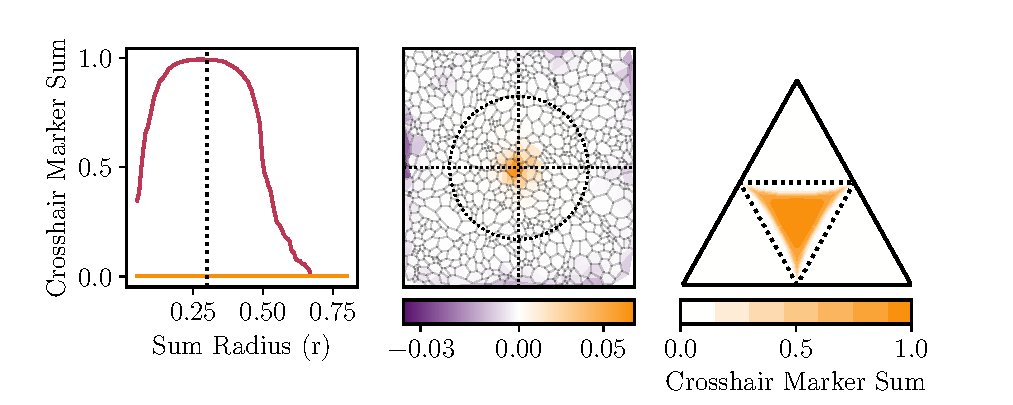
\includegraphics[width=1\textwidth,height=\textheight]{figure_code/amk_chapter/results/phase_diagram_chern/phase_diagram_chern}
\caption[{Local Chern Markers}]{(Center) The crosshair marker~\autocite{peru_preprint}, a local topological marker, evaluated on the Amorphous Kitaev model. The marker is defined around a point, denoted by the dotted crosshair. Information about the local topological properties of the system is encoded within a region around that point. (Left) Summing these contributions up to some finite radius (dotted line here, dotted circle in the centre) gives a generalised version of the Chern number for the system which becomes quantised in the thermodynamic limit. The radius must be chosen large enough to capture information about the local properties of the lattice while not so large as to include contributions from the edge states. The isotropic regime \(J_\alpha = 1\) in red has \(\nu = \pm 1\) implying it supports excitations with non-Abelian statistics, while the anisotropic regime in orange has \(\nu = 0\) implying Abelian statistics. (Right) Extending this analysis to the whole \(J_\alpha\) phase diagram with fixed \(r = 0.3\) nicely confirms that the isotropic phase is non-Abelian.}
\label{fig:phase_diagram_chern}
\end{figure}
}

\hypertarget{edge-modes}{%
\subsubsection{Edge Modes}\label{edge-modes}}

Chiral Spin Liquids support topological protected edge modes on open boundary conditions~\autocite{qi_general_2006}. \Cref{fig:edge_modes} shows the probability density of one such edge mode. It is near zero energy and exponentially localised to the boundary of the system. While the model is gapped in periodic boundary conditions (i.e on the torus) these edge modes appear in the gap when the boundary is cut.

The localisation of the edge modes can be quantified by their inverse participation ratio (IPR) and its scaling with system size \(\tau\), \[\mathrm{IPR} = \int d^2r|\psi(\mathbf{r})|^4  \propto L^{-\tau},\] where \(L\sim\sqrt{N}\) is the linear dimension of the amorphous lattices. This is relevant because localised in-gap states do not participate in transport and hence do not turn band insulators into conductive metals. It is only when the gap fills with extended states that we get a conductive state.

\hypertarget{fig:edge_modes}{%
\begin{figure}
\centering
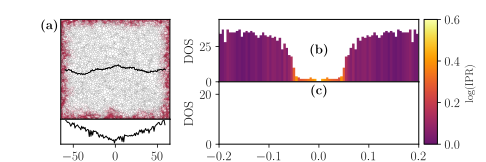
\includegraphics[width=1\textwidth,height=\textheight]{figure_code/amk_chapter/results/edge_modes/edge_modes}
\caption[{Edges States and Density of States}]{(a) The density of one of the topologically protected edge states in the B phase. (Below) the log density plotted along the black path showing that the state is exponentially localised. (a)/(b) The density of states of the corresponding lattice in (a) periodic boundary conditions, (b) open boundary conditions. The colour of the bars shows the mean log IPR for each energy window. Cutting the boundary fills the gap with localised states.}
\label{fig:edge_modes}
\end{figure}
}

\hypertarget{anderson-transition-to-a-thermal-metal}{%
\subsection{Anderson Transition to a Thermal Metal}\label{anderson-transition-to-a-thermal-metal}}

\hypertarget{fig:fermion_gap_vs_L}{%
\begin{figure}
\centering
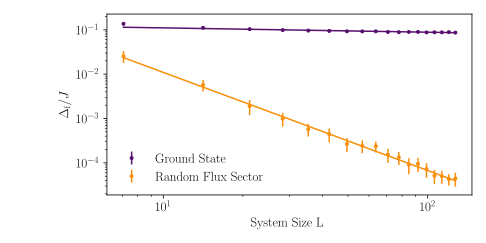
\includegraphics[width=1\textwidth,height=\textheight]{figure_code/amk_chapter/results/fermion_gap_vs_L/fermion_gap_vs_L}
\caption[{Finite Size Scaling of the Fermion Gap}]{Within a flux sector, the fermion gap \(\Delta_f\) measures the energy between the fermionic ground state and the first excited state. This graph shows the fermion gap as a function of system size for the ground state flux sector and for a configuration of random fluxes. We see that the disorder induced by an putting the Kitaev model on an amorphous lattice does not close the gap in the ground state. The gap closing in the flux disordered limit is good evidence that the system transitions to a gapless thermal metal state at high temperature. Each point shows an average over 100 lattice realisations. System size \(L\) is defined \(\sqrt{N}\) where N is the number of plaquettes in the system. Error bars shown are \(3\) times the standard error of the mean. The lines shown are fits of \(\tfrac{\Delta_f}{J} = aL ^ b\) with fit parameters: Ground State: \(a = 0.138 \pm 0.002, b = -0.0972 \pm 0.004\) Random Flux Sector: \(a = 1.8 \pm 0.2, b = -2.21 \pm 0.03\)}
\label{fig:fermion_gap_vs_L}
\end{figure}
}

Previous work on the honeycomb model at finite temperature has shown that the B phase undergoes a thermal transition from a QSL phase to a \emph{thermal metal} phase~\autocite{selfThermallyInducedMetallic2019}. This happens because at finite temperature, thermal fluctuations excite spontaneous vortex-pair formation. As discussed previously, these fluxes are dressed by Majorana bounds states and the composite object is an Ising-type non-Abelian anyon~\autocite{Beenakker2013}. The interactions between these anyons are oscillatory, similar to the Ruderman-Kittel-Kasuya-Yosida (RKKY) exchange and decay exponentially with separation~\autocite{Laumann2012,Lahtinen_2011,lahtinenTopologicalLiquidNucleation2012}. At sufficient density, the anyons hybridise to a macroscopically degenerate state known as \emph{thermal metal}~\autocite{Laumann2012}. At close range the oscillatory behaviour of the interactions can be modelled by a random sign which forms the basis for a random matrix theory description of the thermal metal state.

The amorphous chiral spin liquid undergoes the same Anderson transition to a thermal metal state. Markov Chain Monte Carlo would be necessary to simulate this in full detail~\autocite{selfThermallyInducedMetallic2019} but in order to avoid that complexity in the current work we instead opted to use vortex density \(\rho\) as a proxy for temperature. We give each plaquette the probability \(\rho\) of being a vortex, possibly with one additional adjustment to preserve overall vortex parity. This approximation is exact in the limits \(T = 0\) (corresponding to \(\rho = 0\)) and \(T \to \infty\) (corresponding to \(\rho = 0.5\)) while at intermediate temperatures there may be vortex-vortex correlations that are not captured by our uncorrelated vortex placement.

First, we performed a finite size scaling to check that the presence of a gap in the CSL ground state and absence of a gap in the thermal metal phase are both robust as we go to larger systems, see \cref{fig:fermion_gap_vs_L}. Next we evaluated the fermionic density of states (DOS), Inverse Participation Ratio and IPR scaling exponent \(\tau\) as functions of the vortex density \(\rho\), see \cref{fig:DOS_vs_rho}. This leads to a nice picture of what happens as we raise the temperature of the system away from the gapped, insulating CSL phase. At small \(\rho\), states begin to populate the gap but they have \(\tau\approx0\), indicating that they are localised states pinned to the vortices, and the system remains insulating. At large \(\rho\), the in-gap states merge with the bulk band and become extensive, closing the gap, and the system transitions to the thermal metal phase.

\hypertarget{fig:DOS_vs_rho}{%
\begin{figure}
\centering
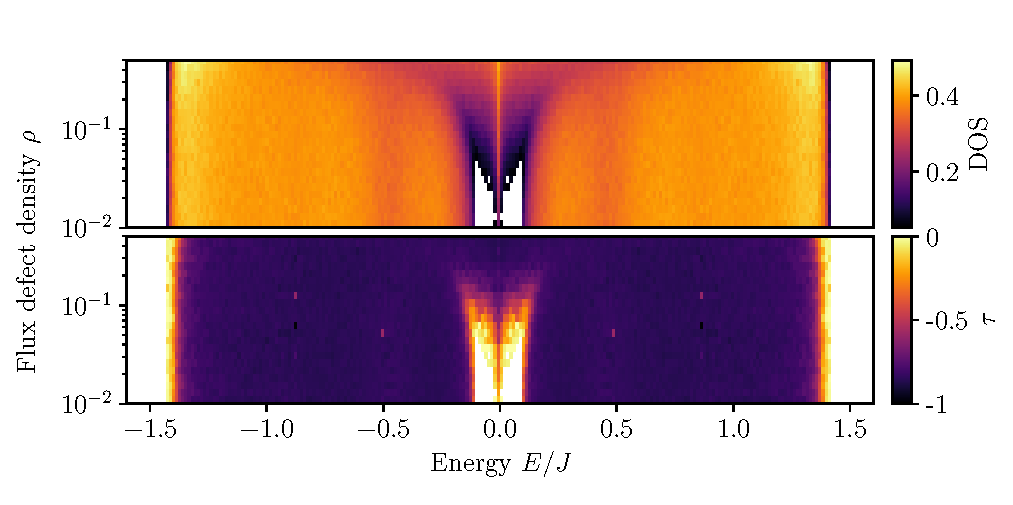
\includegraphics[width=1\textwidth,height=\textheight]{figure_code/amk_chapter/results/DOS_vs_rho/DOS_vs_rho}
\caption[{Transition to a Thermal Metal}]{(Top) Density of states and (Bottom) scaling exponent \(\tau\) of the amorphous Kitaev model as a vortex density \(\rho\) is increased. The scaling exponent \(\tau\) is the exponent with which the inverse participation ratio scales with system size. It gives a measure of the degree of localisation of the states in each \((E/J, \rho)\) bin. At zero \(\rho\) we have the gapped ground state. At small \(\rho\), states begin to populate the gap. These states have \(\tau\approx0\), indicating that they are localised states pinned to fluxes, and the system remains insulating. As \(\rho\) increases further, the in-gap states merge with the bulk band and become extensive, fully closing the gap, and the system transitions to a thermal metal phase.}
\label{fig:DOS_vs_rho}
\end{figure}
}

The thermal metal phase has a signature logarithmic divergence at zero energy and oscillations in the DOS. These signatures can be shown to occur by a recursive argument that involves mapping the original model onto a Majorana model with interactions that take random signs which can itself be mapped onto a coarser lattice with lower energy excitations and so on. This can be repeating indefinitely, showing the model must have excitations at arbitrarily low energies in the thermodynamic limit~\autocite{bocquet_disordered_2000,selfThermallyInducedMetallic2019}. These signatures are shown in \cref{fig:DOS_oscillations} for our model and for the KH model. They do not occur in the KH model unless the chiral symmetry is broken by a magnetic field.

\hypertarget{fig:DOS_oscillations}{%
\begin{figure}
\centering
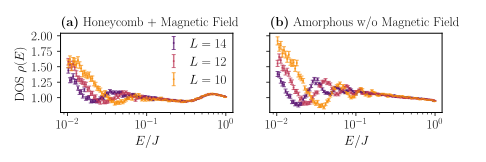
\includegraphics[width=1\textwidth,height=\textheight]{figure_code/amk_chapter/results/DOS_oscillations/DOS_oscillations}
\caption[{Distinctive Oscillations in the Density of States}]{Density of states at high temperature showing the logarithmic divergence at zero energy and oscillations characteristic of the thermal metal state~\autocite{bocquet_disordered_2000,selfThermallyInducedMetallic2019}. (a) shows the honeycomb lattice model in the B phase with magnetic field, while (b) shows that our model transitions to a thermal metal phase without an external magnetic field but rather due to the spontaneous chiral symmetry breaking. In both plots the density of vortices is \(\rho = 0.5\) corresponding to the \(T = \infty\) limit.}
\label{fig:DOS_oscillations}
\end{figure}
}

\hypertarget{sec:AMK-Conclusion}{%
\section{Discussion and Conclusion}\label{sec:AMK-Conclusion}}

In this chapter we have looked at an extension of the KH model to amorphous lattices with coordination number three. We discussed a method to construct arbitrary trivalent lattices using Voronoi partitions, how to embed them onto the torus and how to edge-colour them using a SAT solver. We showed numerically that the ground state flux sector of the model is given by a simple extension of Lieb's theorem. The model has two gapped QSL phases. The two phases support excitations with different anyonic statistics, Abelian and non-Abelian, distinguished using a real-space generalisation of the Chern number~\autocite{peru_preprint}. The presence of odd-sided plaquettes in the model resulted in spontaneous breaking of time reversal symmetry, leading to the emergence of a chiral spin liquid phase. Finally we showed evidence that the amorphous system undergoes an Anderson transition to a thermal metal phase, driven by the proliferation of vortices with increasing temperature. The AK model is an exactly solvable model of the chiral QSL state, one of the first models to exhibit a topologically non-trivial quantum many-body phase on an amorphous lattice. As such this study provides a number of future lines of research.

\hypertarget{experimental-realisations-and-signatures}{%
\subsubsection{Experimental Realisations and Signatures}\label{experimental-realisations-and-signatures}}

We should consider whether a physical amorphous system that supports a QSL ground state could exist. The search for translation invariant Kitaev systems is already motivated by the prospect of a physically realised QSL state, Majorana fermions and direct access to a system with emergent \(\mathbb{Z}_2\) gauge physics~\autocite{TrebstPhysRep2022}. In addition to all this, an amorphous Kitaev model would provide the possibility of exploring the CSL state and potentially very different routes to a physical realisation. One route would be to ask if any crystalline Kitaev material candidates can be heated and rapidly quenched~\autocite{Weaire1976,Petrakovski1981,Kaneyoshi2018} to produce amorphous analogues that might preserve enough of their local structure to support a QSL state.

Considering more designer materials, metal organic frameworks (MOFs) could present a platform for a synthetic Kitaev material. These materials are composed of repeating units of large organic molecules coordinated with metal ions. Amorphous MOFs can be generated with mechanical processes that introduce disorder into crystalline MOFs~\autocite{bennett2014amorphous} and there have been recent proposals for realising strong Kitaev interactions~\autocite{yamadaDesigningKitaevSpin2017} in them as potential signatures of a resonating valence bond QSL state in MOFs with Kagome geometry~\autocite{misumiQuantumSpinLiquid2020}. Finally, MOFs are composed of large synthetic molecules so may provide more opportunity for fine tuning to target particular physics than with ionic compounds. There have also been proposals to realise Kitaev physics in optical lattice experiments~\autocite{duanControllingSpinExchange2003,micheliToolboxLatticespinModels2006} which can also support amorphous lattices~\autocite{sadeghiAmorphousTwodimensionalOptical2005}.

A physical realisation in either an amorphous compound or a MOF would likely incorporate a considerable density of defects. Amorphous silicon, for instance, tends to contain dangling bonds which must be passivated by hydrogenation to improve its physical properties~\autocite{streetHydrogenatedAmorphousSilicon1991}. In both cases, if we assume that Kitaev physics can be realised by crystalline systems, it is not clear if the necessary superexchange couplings would survive the addition of disorder to the lattice. It would therefore make sense theoretically to examine how robust the CSL ground state of the AK model is to additional disorder in the Hamiltonian, for example mis-colourings of the bonds, vertex degree disorder and disorder in coupling strengths. Relatedly, one could look at perturbations to the Hamiltonian that break integrability~\autocite{Rau2014,Chaloupka2010,Chaloupka2013,Chaloupka2015,Winter2016}.

Considering experimental signatures, we expect that the chiral amorphous QSL will display a half-quantised thermal Hall effect similar to the magnetic field induced behaviour of KH materials~\autocite{Kasahara2018,Yokoi2021,Yamashita2020,Bruin2022}. Alternatively, the CSL state could be characterised by local probes such as spin-polarised scanning tunnelling microscopy~\autocite{Feldmeier2020,Konig2020,Udagawa2021} while the thermal metal phase displays characteristic longitudinal heat transport signatures~\autocite{Beenakker2013}. Local perturbations, such as those that might come from an atomic force microscope, could potentially be used to create and control vortices~\autocite{jangVortexCreationControl2021}. To this end, one could look at how the move to amorphous lattices affects vortex time dynamics in perturbed KH models~\autocite{joyDynamicsVisonsThermal2022}.

Given the lack of unambiguous signatures of the QSL state, it can be hard to distinguish the effects of the QSL state from the effect of disorder. So introducing topological disorder may only increase the experimental challenges. That being said, the presence of topological disorder may suppress competing interactions that would otherwise induce magnetic ordering at zero temperature potentially widening the class of materials that could host a QSL ground state. Alternatively, 3D realisations of the AK model could get around this issue of confusing a QSL with disorder because 3D would be expected to have a true Finite-Temperature Phase Transition (FTPT) to the thermal metal state that could be a useful experimental signature~\autocite{eschmannThermodynamicClassificationThreedimensional2020,OBrienPRB2016}. 3D Kitaev systems can also support CSL ground states~\autocite{mishchenkoChiralSpinLiquids2020}.

\hypertarget{thermodynamics}{%
\subsubsection{Thermodynamics}\label{thermodynamics}}

The KH model can be extended to 3D either on trivalent lattices~\autocite{eschmannThermodynamicClassificationThreedimensional2020,OBrienPRB2016} or it can be generalised to an exactly solvable spin-\(\tfrac{3}{2}\) model on 3D four-coordinate lattices~\autocite{yaoAlgebraicSpinLiquid2009,wenQuantumOrderStringnet2003,ryuThreedimensionalTopologicalPhase2009,Baskaran2008,Nussinov2009,Yao2011,Chua2011,Natori2020,Chulliparambil2020,Chulliparambil2021,Seifert2020,WangHaoranPRB2021,Wu2009}. In~\autocite{yaoAlgebraicSpinLiquid2009}, the 2D square lattice with 4 bond types (\(J_w, J_x, J_y, J_z\)) is considered. Since Voronoi partitions in 3D produce lattices of degree four, one interesting generalisation of this work would be to look at the spin-\(\tfrac{3}{2}\) Kitaev model on amorphous lattices.

We did not perform a full Markov Chain Monte Carlo (MCMC) simulation of the AK model at finite temperature but the possible extension to a 3D model with an FTPT would motivate this full analysis. This MCMC simulation would be a numerically challenging task but poses no conceptual barriers~\autocite{Laumann2012,lahtinenTopologicalLiquidNucleation2012,selfThermallyInducedMetallic2019}. Doing this would, first, allow one to look for possible violations of the Harris criterion~\autocite{harrisEffectRandomDefects1974} for the Ising transition of the flux sector. Recall that topological disorder in 2D has radically different properties to that of other kinds of disorder due to the constraints imposed by the Euler equation and maintaining coordination number which allows it to violate otherwise quite general rules like the Harris criterion~\autocite{barghathiPhaseTransitionsRandom2014,schrauthViolationHarrisBarghathiVojtaCriterion2018}. Second, incorporating the projector in addition to MCMC would allow for a full investigation of whether the effect of topological degeneracy is apparent at finite temperatures, this is done for the KH model in~\autocite{selfThermallyInducedMetallic2019}.

Next, one could investigate whether a QSL phase may exist for other models defined on amorphous lattices with a view to more realistic prospects of observation. Do the properties of the Kitaev-Heisenberg model generalise from the honeycomb to the amorphous case?~\autocite{Chaloupka2010,Chaloupka2015,Jackeli2009,Kalmeyer1989,manousakis1991} Alternatively we might look at other lattice construction techniques. For instance we could construct lattices by linking close points~\autocite{agarwala2019topological} or create simplices from random sites~\autocite{christRandomLatticeField1982}. Lattices constructed using these methods would likely have a large number of lattice defects where \(z \neq 3\) in the bulk, leading to many localised Majorana zero modes.

We found a small number of lattices for which Lieb's theorem did not correctly predict the true ground state flux sector. I see two possibilities for what could cause this. Firstly it could be a finite size effect that is amplified by certain rare lattice configurations. It would be interesting to try to elucidate what lattice features are present when Lieb's theorem fails. Alternatively, it might be telling that the ground state conjecture failed in the toric code A phase where the couplings are anisotropic. We showed that the colouring does not matter in the B phase. However an avenue that I did not explore was whether the particular choice of colouring for a lattice affects the physical properties in the toric code A phase. It is possible that some property of the particular colouring chosen is what leads to these rare failures of Lieb's theorem.

Overall, there has been surprisingly little research on amorphous quantum many-body phases despite there being plenty of material candidates. I expect the exact chiral amorphous spin liquid to find many generalisations to realistic amorphous quantum magnets.
